\documentclass[
 size=12pt,
 paper=smartboard, %a4paper, smartboard, screen
 mode=present, %present, handout, print
 display=slides, % slidesnotes, notes, slides
 style=tuliplab,  % TULIP Lab style
 pauseslide,
 fleqn,leqno,clock]{powerdot}

\usepackage{amssymb}
\usepackage{amsmath}
\usepackage{rotating}
\usepackage{graphicx}
\usepackage{boxedminipage}
\usepackage{media9}
\usepackage{rotate}
\usepackage{calc}
\usepackage[absolute]{textpos}
\usepackage{psfrag,overpic}
\usepackage{fouriernc}
\usepackage{pstricks,pst-node,pst-text,pst-3d,pst-grad}
\usepackage{moreverb,epsfig,color,subfigure}
\usepackage{color}
\usepackage{pstricks}
\usepackage{pstricks-add}
\usepackage{pst-text}
\usepackage{pst-node, pst-tree}
\usepackage{booktabs}
\usepackage{etex}
\usepackage{breqn}
\usepackage{multirow}
% \usepackage{pst-rel-points}
\usepackage{listings}
\usepackage{hyperref}
\hypersetup{ % TODO: PDF meta Data
  pdftitle={Presentation Title},
  pdfauthor={Gang Li},
  pdfpagemode={FullScreen},
  pdfborder={0 0 0}
}


% \usepackage{auto-pst-pdf}
% package to show source code

\definecolor{LightGray}{rgb}{0.9,0.9,0.9}
\newlength{\pixel}\setlength\pixel{0.000714285714\slidewidth}
\setlength{\TPHorizModule}{\slidewidth}
\setlength{\TPVertModule}{\slideheight}
\newcommand\highlight[1]{\fbox{#1}}
\newcommand\icite[1]{{\footnotesize [#1]}}

\newcommand\twotonebox[2]{\fcolorbox{pdcolor2}{pdcolor2}{#1\vphantom{#2}}\fcolorbox{pdcolor2}{white}{#2\vphantom{#1}}}
\newcommand\twotoneboxo[2]{\fcolorbox{pdcolor2}{pdcolor2}{#1}\fcolorbox{pdcolor2}{white}{#2}}
\newcommand\vpspace[1]{\vphantom{\vspace{#1}}}
\newcommand\hpspace[1]{\hphantom{\hspace{#1}}}
\newcommand\COMMENT[1]{}

\newcommand\placepos[3]{\hbox to\z@{\kern#1
        \raisebox{-#2}[\z@][\z@]{#3}\hss}\ignorespaces}


%%%%%%%%%%%%%%%%%%%%%%%%%%%%%%%%%%%%%%%%%%%%%%%%%%%%%%%%%%%%%%%%%%%%%%%%%%
%%% title
%%% TODO: Customize to your Own Title, Name, Address
%%%
\title{FLIP(00) Mid-term Presentation}
\author{Rongxin Xu\\
Hunan University
% \href{mailto:gangli@acm.org}{gangli@acm.org}
% \and % more authors
}
\date{26 October 2019}



% Customize the setting of slides
\pdsetup{
% TODO: Customize the left footer, and right footer
rf={\copyright \emph{FLIP(00)}},
cf={FLIP(00) Presentation },
}


% Starts the document
\begin{document}

\maketitle

%%==========================================================================================
%%
\begin{slide}[toc=,bm=]{Outline}
  \tableofcontents[content=sections]
\end{slide}
%%
%%==========================================================================================

\section{Introduction}

\begin{slide}{Problem Description}
  \begin{itemize}
    \item<1->
          This is a problem with time-series prediction.
          There are six data sets with a total of 11 attributes.
          The following is some requirements.
          \begin{itemize}
            \item<2->
                  According to the given train data set,
                  training a model and then using the model to predict total sales for every product and store in the next month.
          \end{itemize}
  \end{itemize}
\end{slide}

\section{Data Description}
%
\begin{slide}{Attribute Information}
  \begin{itemize}
    \item<1->
          Attribute Information
    \item[1.]
          There are six data sets with a total of 11 attributes.
          \begin{figure}
            \centering
            % Requires \usepackage{graphicx}
            \includegraphics[width=4in,height=3in]{Figures/0.eps}
            \caption{Attributes name and description}
            \label{Attributes name and description}
          \end{figure}
    \item[2.]
          The detailed description of the data is shown in the following table.
  \end{itemize}
\end{slide}

\begin{slide}{Detailed description}
  \begin{figure}[htbp]
    \centering
    \subfigure[sales_train.csv]{
      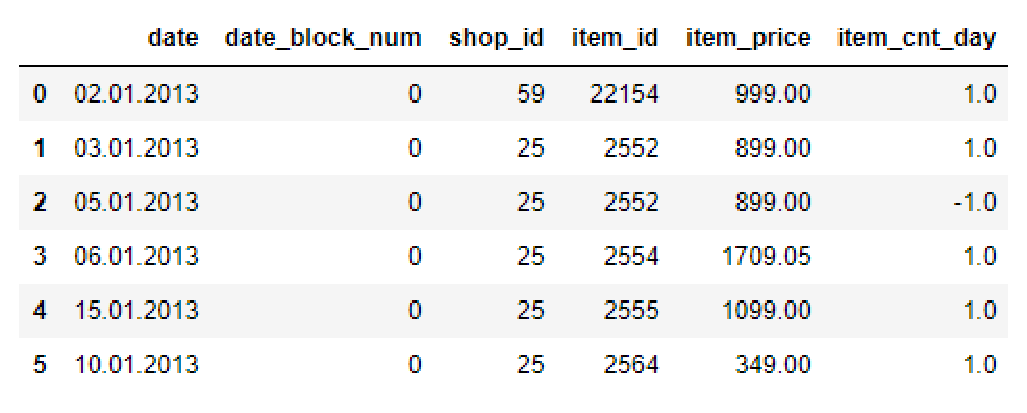
\includegraphics[width=7cm]{Figures/1.eps}
      %\caption{fig1}
    }
    \quad
    \subfigure[item_categories.csv]{
      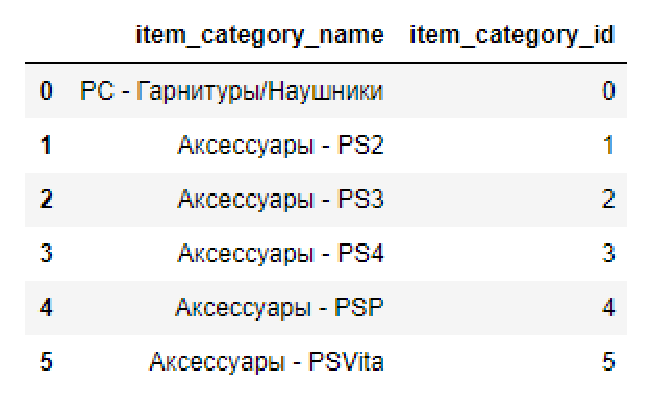
\includegraphics[width=5cm]{Figures/2.eps}
    }
    \quad
    \subfigure[test.csv]{
      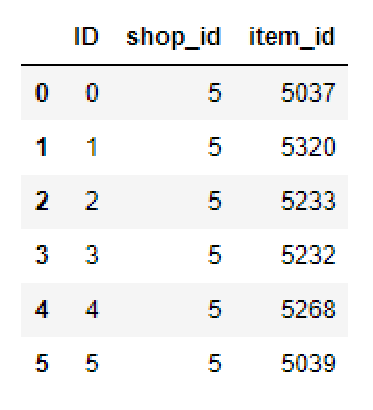
\includegraphics[width=3cm]{Figures/5.eps}
    }
    \quad
    \subfigure[items.csv]{
      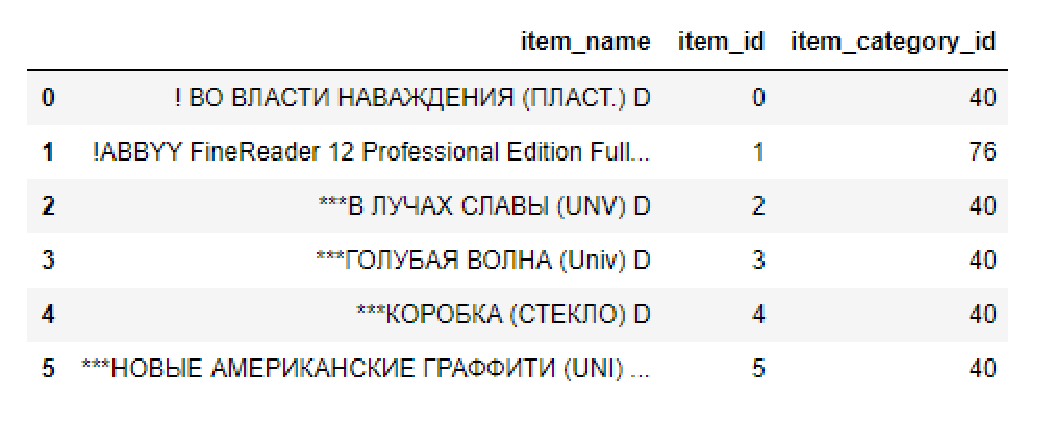
\includegraphics[width=7cm]{Figures/3.eps}
    }
    \quad
    \subfigure[shops.csv]{
      \includegraphics[width=4cm]{Figures/4.eps}
    }
    \caption{Data Description}
  \end{figure}
\end{slide}

\begin{slide}{Summary}
  \begin{itemize}
    \item
          The data is very clean and complete,
          so we only need to change the data type after importing.
    \item
          We also need to reorganize the table structure to make it more readable.
          An sample is given below.
          \begin{figure}
            \centering
            % Requires \usepackage{graphicx}
            \includegraphics[width=4in,height=3in]{Figures/13.eps}
            \caption{sample}
            \label{sample}
          \end{figure}
  \end{itemize}
\end{slide}

\section{Exploratory Data Analysis}

\begin{slide}{Exploratory Data Analysis}
  \begin{figure}[htbp]
    \centering
    \subfigure[Items per Category]{
      \includegraphics[width=7cm]{Figures/6.eps}
      %\caption{fig1}
    }
    \quad
    \subfigure[Total Sales of the company]{
      \includegraphics[width=9cm]{Figures/7.eps}
    }
    \quad
    \subfigure[Rolling Mean and std]{
      \centering
      \includegraphics[width=12cm]{Figures/8.eps}
    }
    \caption{EDA}
  \end{figure}
\end{slide}

\begin{slide}{Summary}
  \begin{itemize}
    \item
          There is an obvious "seasonality" (Eg: peak sales around a time of year)
          and a decreasing "Trend".
  \end{itemize}
\end{slide}

\section{Stationarity}

\begin{slide}{Seasonality and Trend}
  \begin{figure}
    \centering
    % Requires \usepackage{graphicx}
    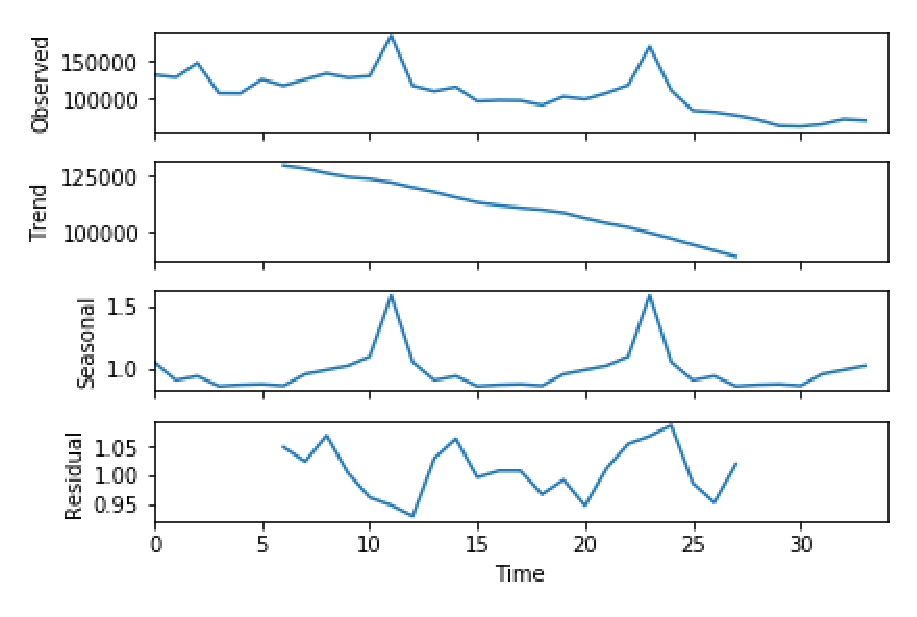
\includegraphics[width=5in]{Figures/9.eps}
    \caption{Seasonality and Trend}
    \label{Seasonality and Trend}
  \end{figure}
\end{slide}

\begin{slide}{Stationarity Test}
  \begin{figure}
    \centering
    % Requires \usepackage{graphicx}
    \includegraphics[width=4in]{Figures/10.eps}
    \caption{Stationarity Test}
    \label{Stationarity Test}
  \end{figure}
\end{slide}

\begin{slide}{Remove seasonality and trends}
  \begin{figure}
    \centering
    % Requires \usepackage{graphicx}
    \includegraphics[width=6in,height=4in]{Figures/11.eps}
    \caption{Remove seasonality and trends}
    \label{Remove seasonality and trends}
  \end{figure}
\end{slide}

\begin{slide}{Summary}
  \begin{itemize}
    \item
          Now let's check the new P-value.
          \begin{figure}
            \centering
            % Requires \usepackage{graphicx}
            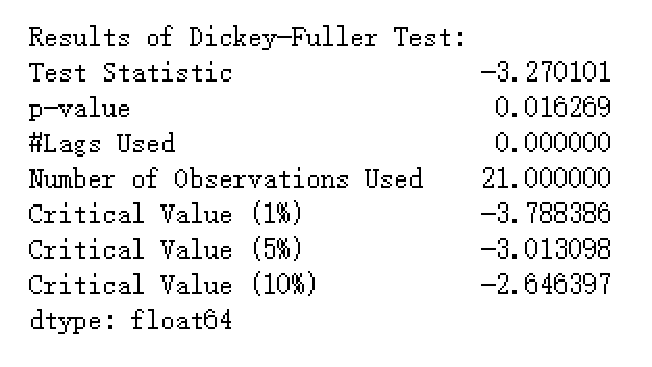
\includegraphics[width=3in,height=2in]{Figures/12.eps}
            \caption{new stationarity test}
            \label{new stationarity test}
          \end{figure}
    \item
          After the transformations, our p-value for the DF test is well within 0.05.
          Hence we can assume Stationarity of the series.
  \end{itemize}
\end{slide}

\section{Conclusion}
\begin{slide}{Summary}
  \begin{itemize}
    \item From the above result presentation, we can find that
          \subitem There are seasonality and trend in data.
          \bigskip
    \item From the Stationarity test, we can find that
          \subitem After removing seasonality and trends, the time series becomes smooth.
          \smallskip
          \subitem So we can use traditional time series prediction methods for prediction.
  \end{itemize}
\end{slide}

\begin{slide}{Future research}
  \begin{itemize}
    \item Predict by traditional time series prediction models such as AR, MA and ARMA.
    \item Using more models to predict, such as random forests and neural networks.
    \item Find the most effective model and get my own kaggle ranking.
  \end{itemize}
\end{slide}

\begin{wideslide}[toc=,bm=]{}
  \centering
  \vspace{\stretch{1}}
  \twocolumn[
    lcolwidth=0.35\linewidth,
    rcolwidth=0.65\linewidth
  ]
  {
    % \centerline{\includegraphics[scale=.2]{tulip-logo.eps}}
  }
  {
    \vspace{\stretch{1}}


    \textcolor{black}{\scalebox{2.0}{Thank you \& Question}}


  }
  \vspace{\stretch{1}}
\end{wideslide}

\end{document}
\endinput
